\section{Results}
Both the monolithic network and the modular network were tested on the following test cases:
\begin{itemize}
\item 5 \times 5 grid world with the subnetworks evolving for 5, 10, 15, 50 generations and the overall network evolving for 100 generations in all cases. This was run for both ESP and NEAT
\item 10 \times 10 grid world with the subnetworks evolving for 5, 10, 15, 50 generations and the overall network evolving for 100 generations in all cases. This was also run for both ESP and NEAT
\item For the case of ESP, the algorithm was run with prey and hunter move probability set to 01, 0.5, 0.7 and 0.8. The number of generations of the sub-network evolution was fixed at 10. The overall network was run for 100 generations. 
\end{itemize}

For the 5 \times 5 gridsize, the maximum number of steps per episode was fixed at 100, while for the 10 \times 10 grid size, it was fixed at 1000. It seems like this value would play an important part in the performance, since it has to be high enough so that the agent gets enough time to get near the prey (which takes longer on larger grids) 

First the experiments were run using NEAT.
Figure \ref{fig:MeanMAPNDCGPI1} a and b show the average predator fitness and the percentage improvement over the monolithic network for the 5x5 grid for the monolithic network, and for the case where the subnetwork was evolved for 50 generations. In this case the monolithic network seems to perform better than the modular network throughout. This might be because of the small size of the environment, which makes it easier for the monolithic network to learn, without having to contend with having to coordinate between the subnetworks. 

Figure \ref{fig:MeanMAPNDCGPI2} show the average predator fitness and the percentage improvement over the monolithic network for the 5x5 grid for the monolithic network, and the cases where the subnetworks were evolved for 5, 10, 15 and 50 generations. Again, the monolithic network is consistently better than the modular networks, and the number of generations the subnetworks were evolved doesn't seem to have a significant effect on the performance, although evolving the subnetwork for 15 generations seems to perform slightly better.

Very similar results are obtained for the 10 \times 10 grid size. The monolithic network performs much better in the case where the subnetwork is evolved for 50 generations (Figure \ref{fig:MeanMAPNDCGPI3}) and for cases where the subnetwork is evolved for 5, 10, 15 and 50 generations (Figure \ref{fig:MeanMAPNDCGPI4}).

Figures \ref{fig:MeanMAPNDCGPI5}, \ref{fig:MeanMAPNDCGPI6}, \ref{fig:MeanMAPNDCGPI7} and \ref{fig:MeanMAPNDCGPI8} show the values of the fitness of the champion for the respective cases. Comparing the fitness values of the champions in these figures with the average fitness values in the previous 4 figures, one can see that the fitness of the champion is an order of magnitude higher than the average. And since this is a plot of one agent, the champion, there is more variation in the fitness. But overall, the same trend holds -- the monolithic network performs better than or as good as the modular network in all cases. 

Since in NEAT, the entire overall network, including the subnetworks (seeded from the separate subtasks) are evolved in the overall task, it is possible that the network has more learning to do. It has a larger network, where the entire network is changing. It is possible that if the overall network were evolved for more generations, it might eventually perform better than the monolithic network.

Figure \ref{fig:MeanMAPNDCGPI9} shows the performance of the various modular networks and the monolithic network that are evolved using ESP for a 5x5 grid world. In Figure \ref{fig:MeanMAPNDCGPI9} a, one can see that the modular networks learn much faster than the monolithic network initially, and although the monolithic network catches up the modular network where the subnetworks were evolved for 5 generations (the green line) out-performs the monolithic network all the time. 

Firstly, it is interesting to note that, while using NEAT, the monolithic network always performed the best, using ESP, the modular networks are almost as competitive. This could be attributed to the fact that, in NEAT when the overall network is evolved for the overall task, the weights of the subnetworks (that were seeded from the subtasks) are also changed, while in the ESP implementation, they are not. So although these results don't really give a fair comparison  between ESP and NEAT, it is interesting to note that fixing the subnetworks and evolving only the coordinating network in the overall network seems to make a difference in performance. 

Secondly, the modular network where the subnetwork was evolved only for 5 generations seems to outperform all the other networks. This might be because, since the gird world is small, anything more than 5 generations for the subtask might over train the network, or maybe the coordination network finds it easier to coordinate between slightly lesser trained subnetworks (which it can over ride easily) rather than well trained subnetworks with strong activation.

Figure \ref{fig:MeanMAPNDCGPI10} shows the performance of ESP for the various modular subnetworks and the monolithic network for a 10x10 grid size. In this case, the monolithic network outperforms all the other networks all the time, although the modular network with the subnetwork evolved for 5 generations seems to be able to keep up with the monolithic network most of the time. Since the grid size is larger the task is proportionally much harder. So for the case of the modular network, it is possible that the coordinating layer on top finds it much harder to coordinate the inputs from the subnetworks. And the modular network with the subnetwork evolved for 5 generations performs as well maybe for the same reason as described in the 5x5 grid size -- the coordinating network has an easier time coordinating slightly lesser trained subnetworks.



%%%%%%%%%%%%%%%%%%%%%%%%%%%%%%%%%%%%
%%%%%% AVERAGE 
%%%%%%%%%%%%%%%%%%%%%%%%%%%%%%%%%%%%
% Average % 5x5 % monolithic and 50
\begin{figure*}
\centering
\subfigure[5x5 Average Fitness]{
  \label{fig:neat_5x5_av_m50}
  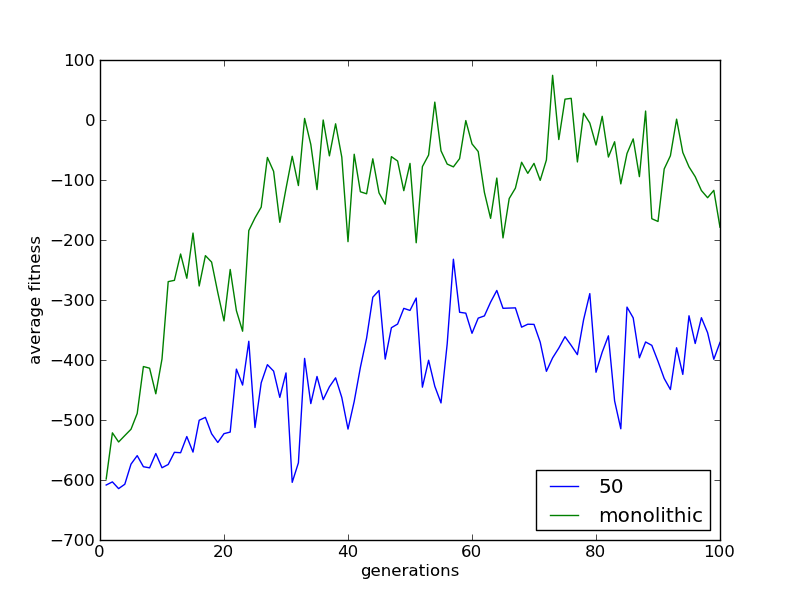
\includegraphics[scale=0.50]{figs/neat/average/5x5/monolithic_and_50/fitness-vs-generations.png}}
\hspace{1in}
\subfigure[5x5 Percent Improvement]{
  \label{fig:neat_5x5_av_m50_pi}
  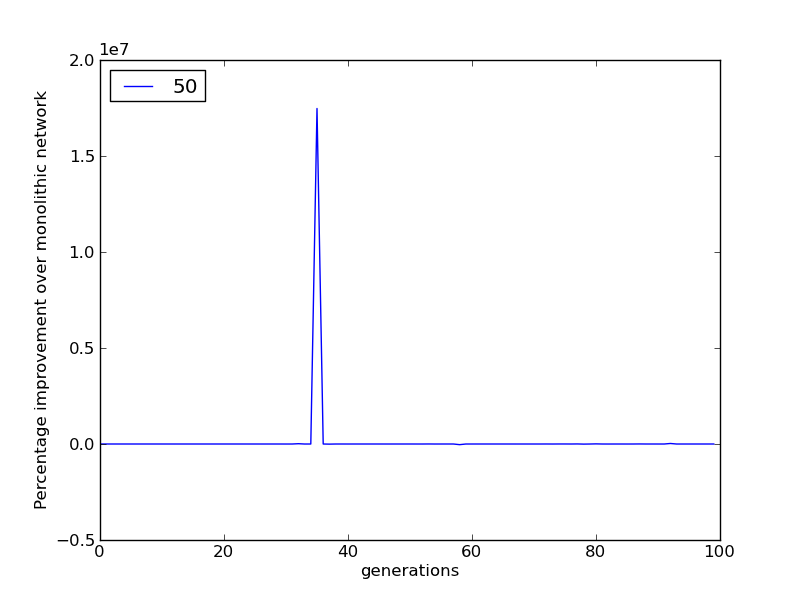
\includegraphics[scale=0.50]{figs/neat/average/5x5/monolithic_and_50/improvement-vs-generations.png}}
  \caption{Average fitness plotted over generations for a 5x5 grid for
  monolithic network and network seeded with modular networks evolved for 50
  generations}
  \label{fig:MeanMAPNDCGPI} % label for entire figure
\end{figure*}

% Average % 5x5 % all 
\begin{figure*}
\centering
\subfigure[5x5 Average Fitness]{
  \label{fig:neat_5x5_av_all}
  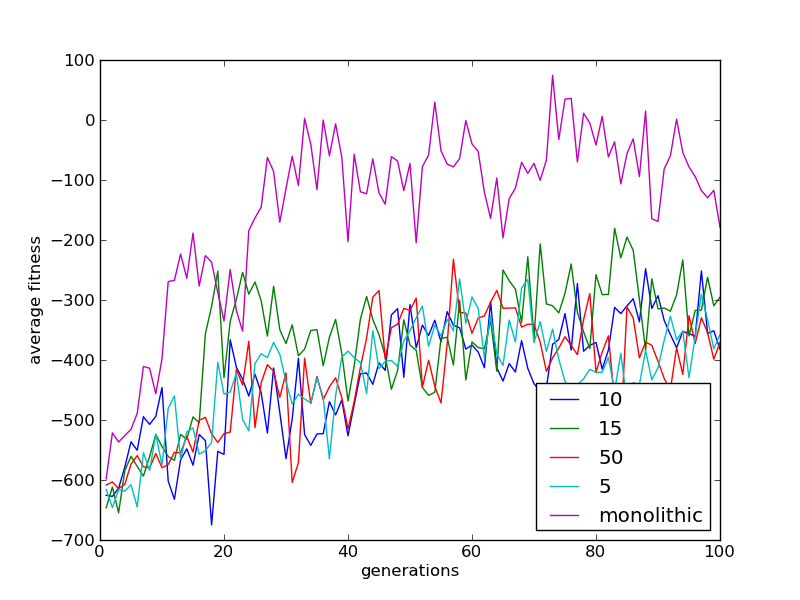
\includegraphics[scale=0.50]{figs/neat/average/5x5/all/fitness-vs-generations.png}}
\hspace{1in}
\subfigure[5x5 Percent Improvement]{
  \label{fig:neat_5x5_av_all_pi}
  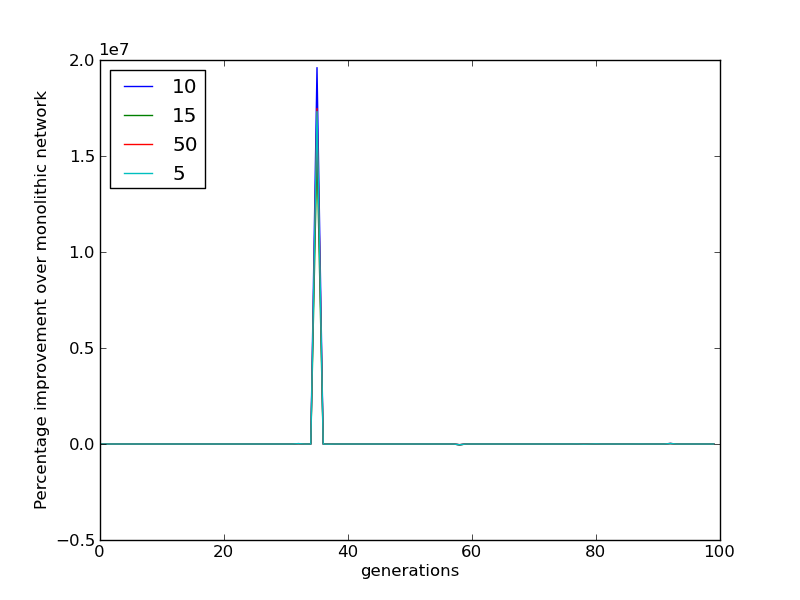
\includegraphics[scale=0.50]{figs/neat/average/5x5/all/improvement-vs-generations.png}}
  \caption{Average fitness plotted over generations for a 5x5 grid for
  monolithic network and network seeded with modular networks evolved for 5,
  10, 15 and 50 generations}
  \label{fig:MeanMAPNDCGPI} % label for entire figure
\end{figure*}

% Average % 10x10 % monolithic and 50
\begin{figure*}
\centering
\subfigure[10x10 Average Fitness]{
  \label{fig:neat_10x10_av_m50}
  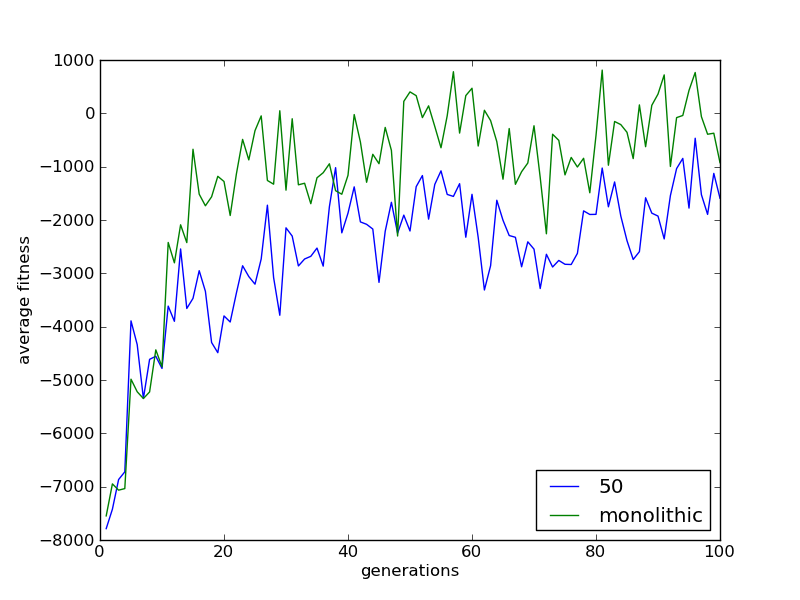
\includegraphics[scale=0.50]{figs/neat/average/10x10/monolithic_and_50/fitness-vs-generations.png}}
\hspace{1in}
\subfigure[10x10 Percent Improvement]{
  \label{fig:neat_10x10_av_m50_pi}
  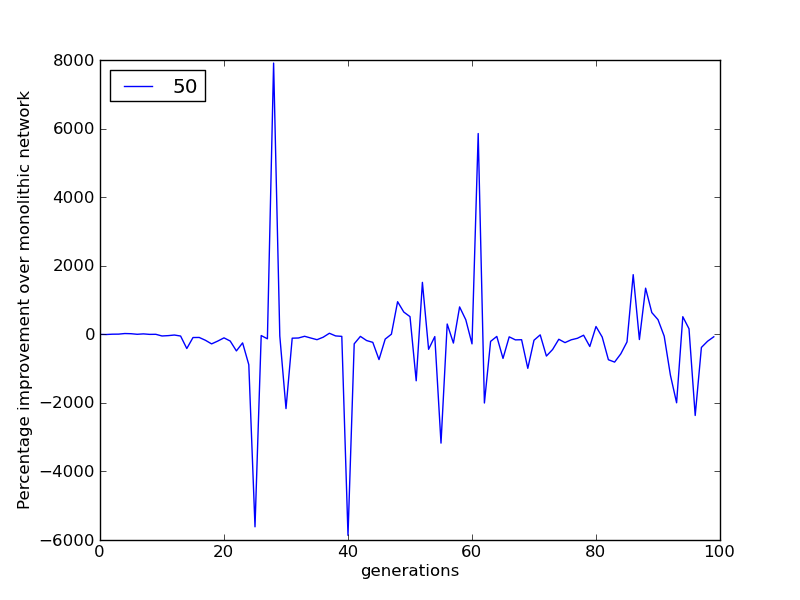
\includegraphics[scale=0.50]{figs/neat/average/10x10/monolithic_and_50/improvement-vs-generations.png}}
  \caption{Average fitness plotted over generations for a 10x10 grid for
  monolithic network and network seeded with modular networks evolved for 50
  generations}
  \label{fig:MeanMAPNDCGPI} % label for entire figure
\end{figure*}

% Average % 10x10 % all 
\begin{figure*}
\centering
\subfigure[10x10 Average Fitness]{
  \label{fig:neat_10x10_av_all}
  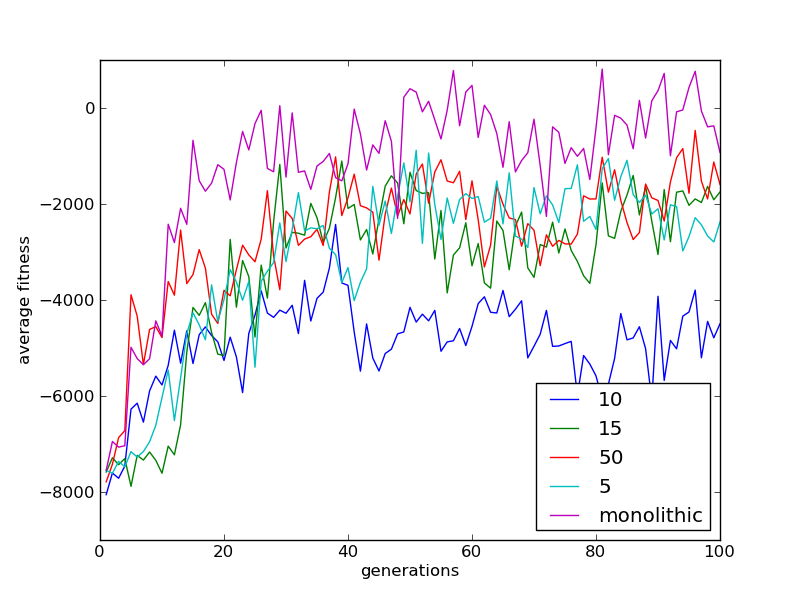
\includegraphics[scale=0.50]{figs/neat/average/10x10/all/fitness-vs-generations.png}}
\hspace{1in}
\subfigure[10x10 Percent Improvement]{
  \label{fig:neat_10x10_av_all_pi}
  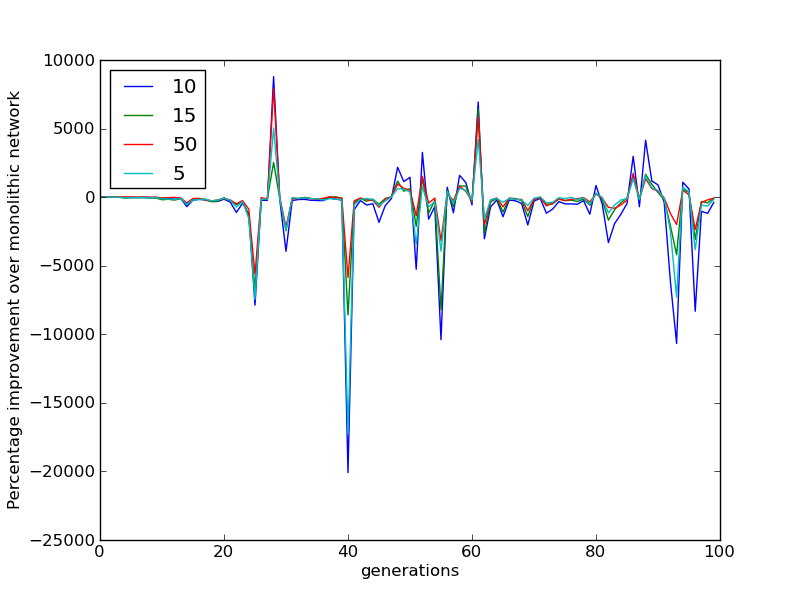
\includegraphics[scale=0.50]{figs/neat/average/10x10/all/improvement-vs-generations.png}}
  \caption{Average fitness plotted over generations for a 10x10 grid for
  monolithic network and network seeded with modular networks evolved for 5,
  10, 15 and 50 generations}
  \label{fig:MeanMAPNDCGPI} % label for entire figure
\end{figure*}

%%%%%%%%%%%%%%%%%%%%%%%%%%%%%%%%%%%%
%%%%%% CHAMPION
%%%%%%%%%%%%%%%%%%%%%%%%%%%%%%%%%%%%
% Champion % 5x5 % monolithic and 50
\begin{figure*}
\centering
\subfigure[5x5 Champion Fitness]{
  \label{fig:neat_5x5_c_m50}
  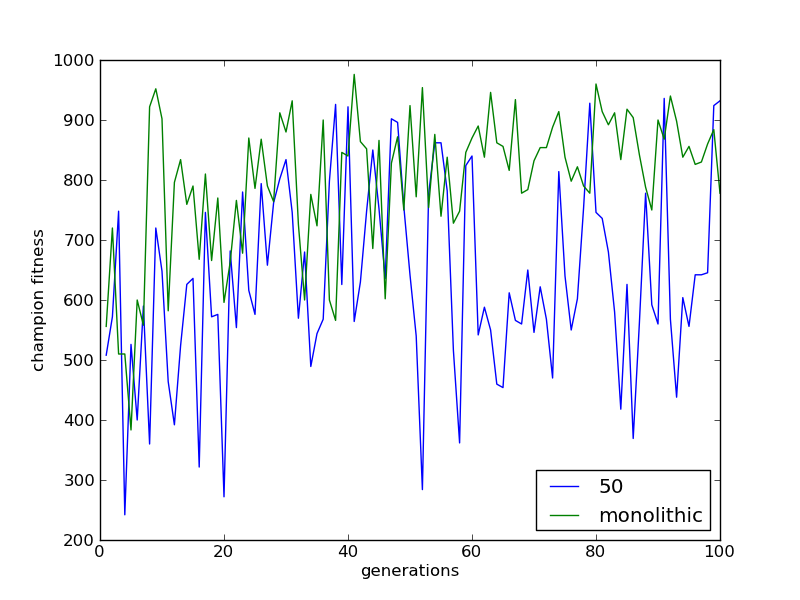
\includegraphics[scale=0.50]{figs/neat/champion/5x5/monolithic_and_50/fitness-vs-generations.png}}
\hspace{1in}
\subfigure[5x5 Percent Improvement]{
  \label{fig:neat_5x5_c_m50_pi}
  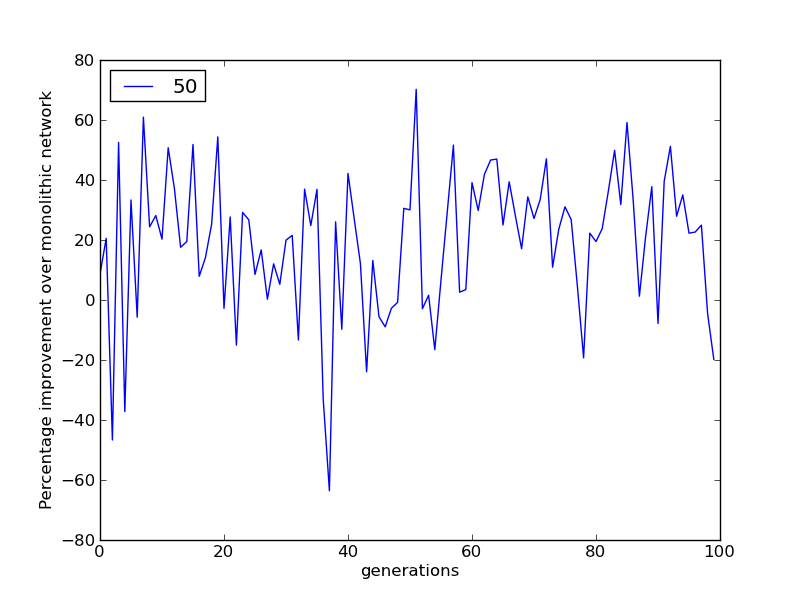
\includegraphics[scale=0.50]{figs/neat/champion/5x5/monolithic_and_50/improvement-vs-generations.png}}
  \caption{Champion fitness plotted over generations for a 5x5 grid for
  monolithic network and network seeded with modular networks evolved for 50
  generations}
  \label{fig:MeanMAPNDCGPI} % label for entire figure
\end{figure*}

% Champion % 5x5 % all 
\begin{figure*}
\centering
\subfigure[5x5 Champion Fitness]{
  \label{fig:neat_5x5_c_all}
  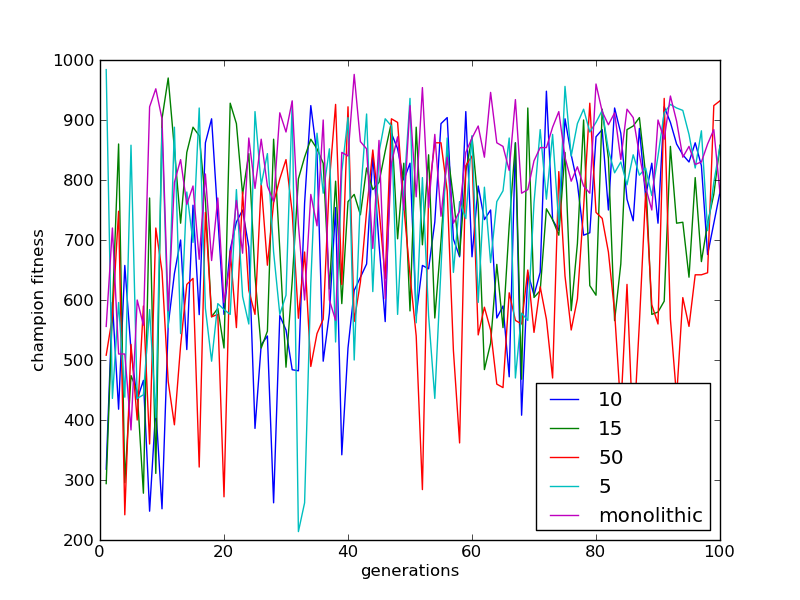
\includegraphics[scale=0.50]{figs/neat/champion/5x5/all/fitness-vs-generations.png}}
\hspace{1in}
\subfigure[5x5 Percent Improvement]{
  \label{fig:neat_5x5_c_all_pi}
  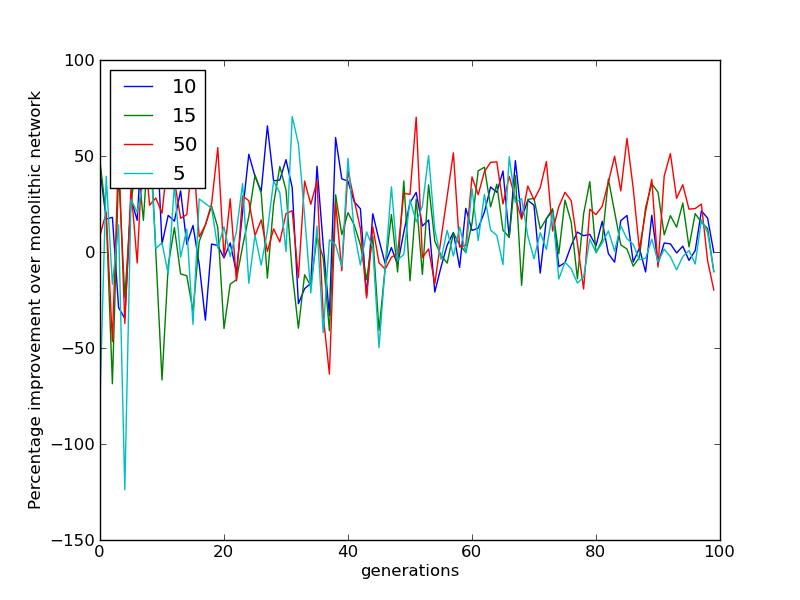
\includegraphics[scale=0.50]{figs/neat/champion/5x5/all/improvement-vs-generations.png}}
  \caption{Champion fitness plotted over generations for a 5x5 grid for
  monolithic network and network seeded with modular networks evolved for 5,
  10, 15 and 50 generations}
  \label{fig:MeanMAPNDCGPI} % label for entire figure
\end{figure*}

% Champion % 10x10 % monolithic and 50
\begin{figure*}
\centering
\subfigure[10x10 Champion Fitness]{
  \label{fig:neat_10x10_c_m50}
  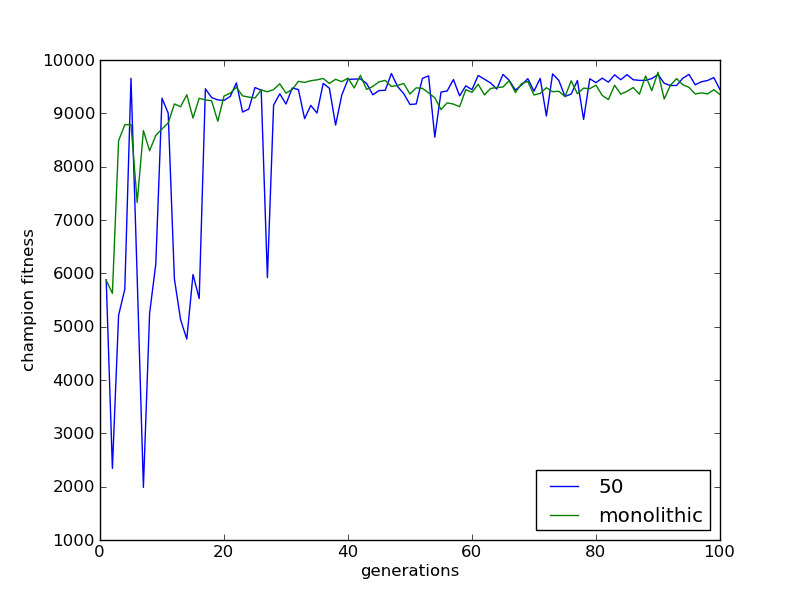
\includegraphics[scale=0.50]{figs/neat/champion/10x10/monolithic_and_50/fitness-vs-generations.png}}
\hspace{1in}
\subfigure[10x10 Percent Improvement]{
  \label{fig:neat_10x10_c_m50_pi}
  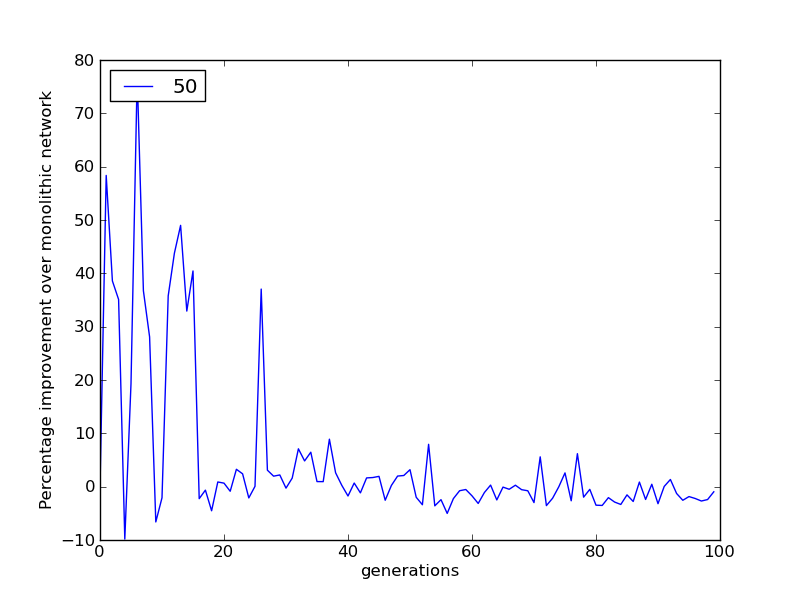
\includegraphics[scale=0.50]{figs/neat/champion/10x10/monolithic_and_50/improvement-vs-generations.png}}
  \caption{Champion fitness plotted over generations for a 10x10 grid for
  monolithic network and network seeded with modular networks evolved for 50
  generations}
  \label{fig:MeanMAPNDCGPI} % label for entire figure
\end{figure*}

% Champion % 10x10 % all 
\begin{figure*}
\centering
\subfigure[10x10 Champion Fitness]{
  \label{fig:neat_10x10_c_all}
  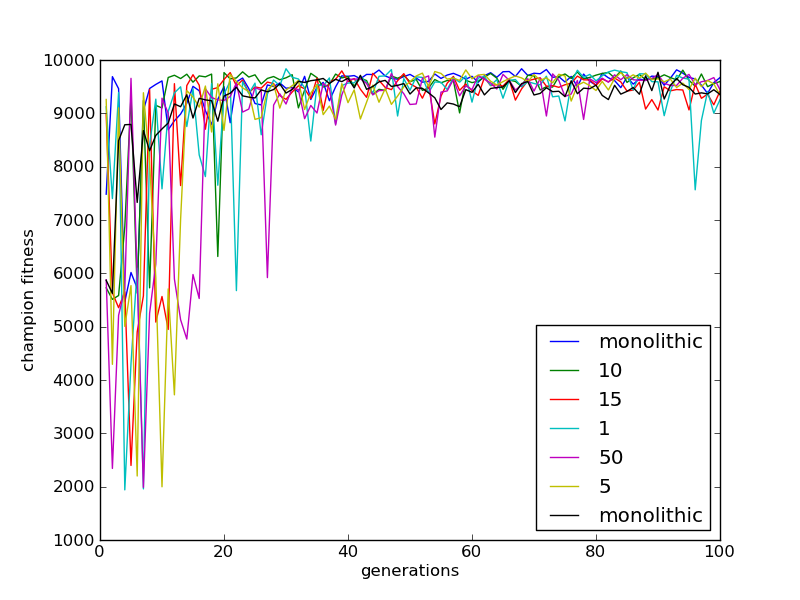
\includegraphics[scale=0.50]{figs/neat/champion/10x10/all/fitness-vs-generations.png}}
\hspace{1in}
\subfigure[10x10 Percent Improvement]{
  \label{fig:neat_10x10_c_all_pi}
  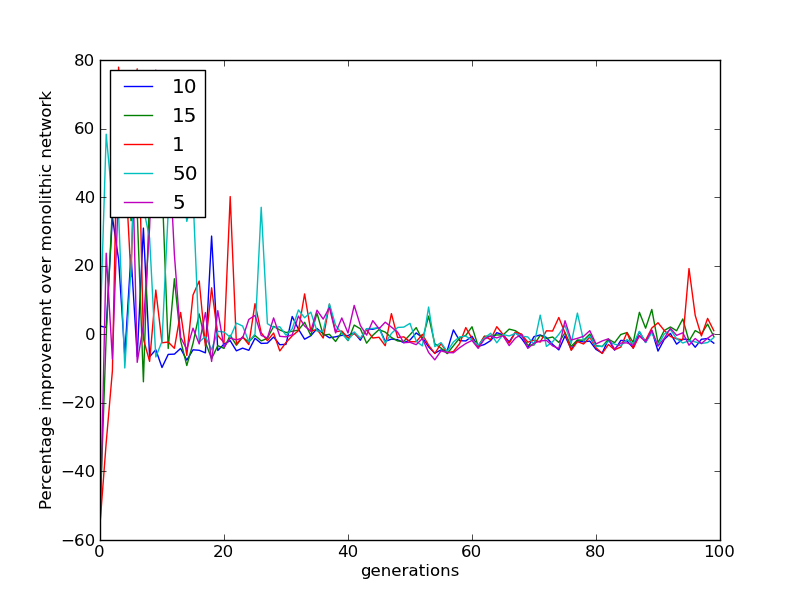
\includegraphics[scale=0.50]{figs/neat/champion/10x10/all/improvement-vs-generations.png}}
  \caption{Champion fitness plotted over generations for a 10x10 grid for
  monolithic network and network seeded with modular networks evolved for 5,
  10, 15 and 50 generations}
  \label{fig:MeanMAPNDCGPI} % label for entire figure
\end{figure*}

%%%%%%%%%%%%%%%%%%%%%%%%%%%%%%%%%%%%
%%%%%% AVERAGE 
%%%%%%%%%%%%%%%%%%%%%%%%%%%%%%%%%%%%
% Average % 5x5 % monolithic and all 
\begin{figure*}
\centering
\subfigure[5x5 Average Fitness]{
  \label{fig:esp_5x5_av_all}
  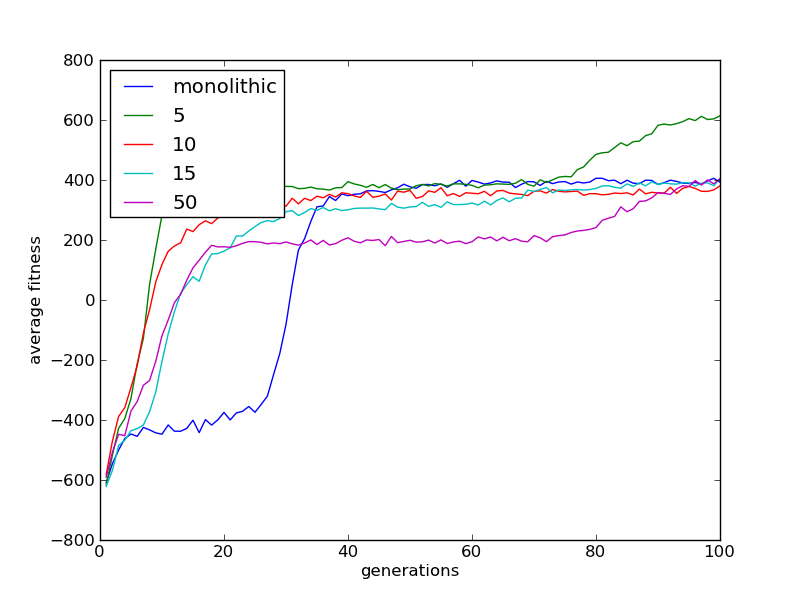
\includegraphics[scale=0.50]{figs/esp/fitness-vs-generations-5x5.png}}
\hspace{1in}
\subfigure[5x5 Percent Improvement]{
  \label{fig:esp_5x5_av_all_pi}
  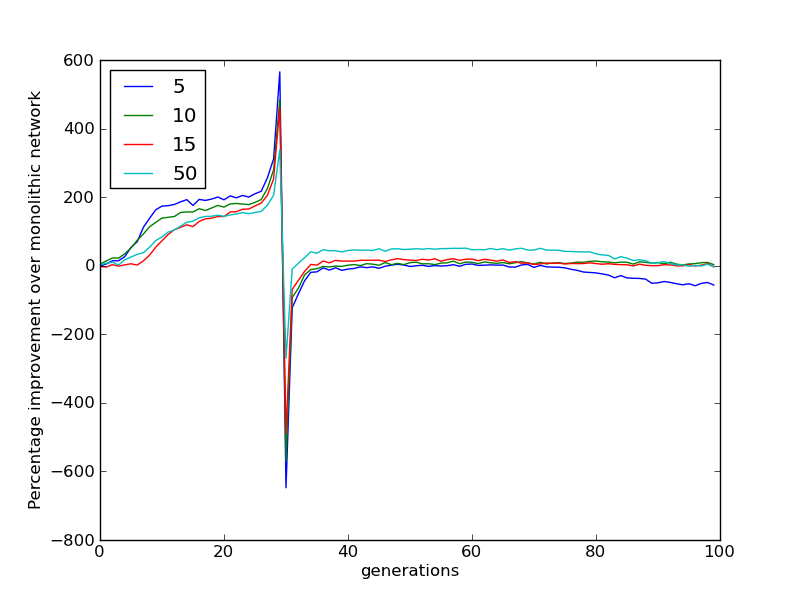
\includegraphics[scale=0.50]{figs/esp/improvement-vs-generations-5x5.png}}
  \caption{ESP: Average fitness plotted over generations for a 5x5 grid for
  monolithic network and network seeded with modular networks evolved for 5, 10, 15 and 50
  generations}
  \label{fig:MeanMAPNDCGPI9} % label for entire figure
\end{figure*}

% Average % 10x10 % monolithic and all 
\begin{figure*}
\centering
\subfigure[10x10 Average Fitness]{
  \label{fig:esp_10x10_av_all}
  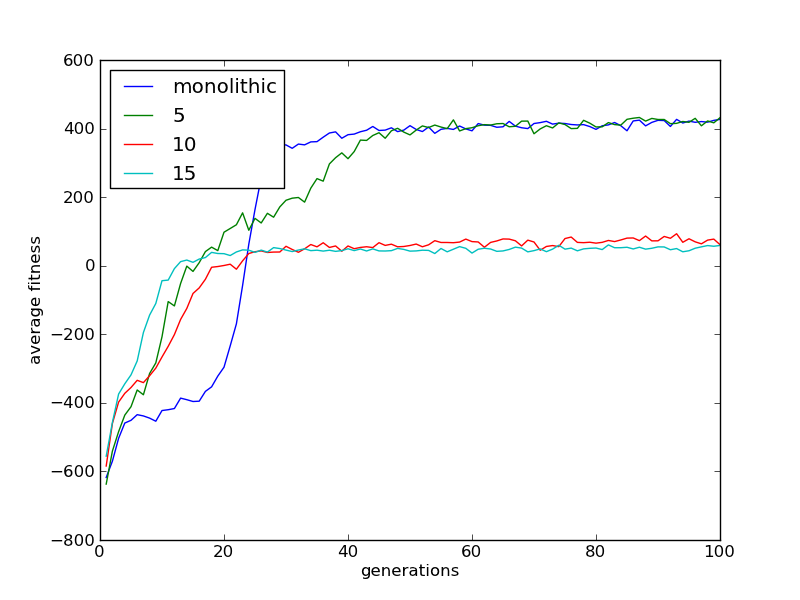
\includegraphics[scale=0.50]{figs/esp/fitness-vs-generations-10x10.png}}
\hspace{1in}
\subfigure[5x5 Percent Improvement]{
  \label{fig:esp_10x10_av_all_pi}
  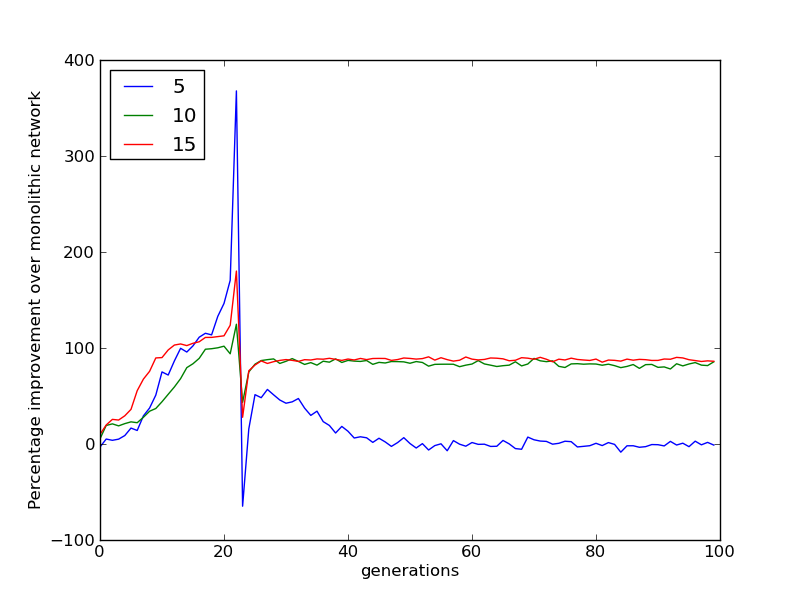
\includegraphics[scale=0.50]{figs/esp/improvement-vs-generations-10x10.png}}
  \caption{ESP: Average fitness plotted over generations for a 10x10 grid for
  monolithic network and network seeded with modular networks evolved for 5, 10, 15 and 50
  generations}
  \label{fig:MeanMAPNDCGPI10} % label for entire figure
\end{figure*}

% fitness-vs-generations-probs.png
\begin{figure*}[htp]
	\centering
	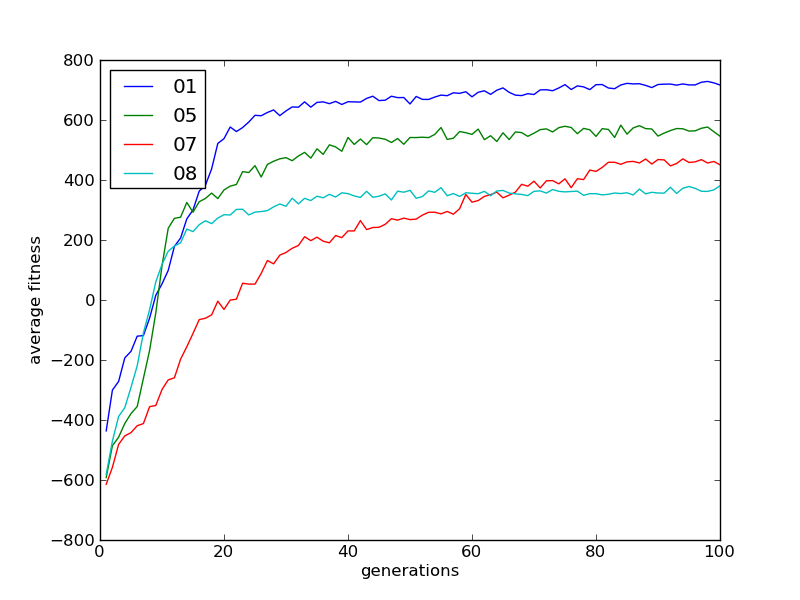
\includegraphics[scale=0.50]{figs/esp/fitness-vs-generations-probs.png}
	\caption{Performance of modular approach on a 5x5 grid with different move probabilities (0.1, 0.5, 0.7, 0,8) of hunter and prey (values for both are set to be the same)}
	\label{fig:MAPPIAll11}
\end{figure*}

